\documentclass[twoside,twocolumn]{article}

\usepackage{blindtext} 
\usepackage{graphicx}
\usepackage[sc]{mathpazo} 
\usepackage[T1]{fontenc} 
\linespread{1.05} 
\usepackage{microtype} 


\usepackage[english]{babel} 


\usepackage[hmarginratio=1:1,top=32mm,columnsep=20pt]{geometry} 
\usepackage[hang, small,labelfont=bf,up,textfont=it,up]{caption} 
\usepackage{booktabs} 


\usepackage{lettrine} 


\usepackage{enumitem} 
\setlist[itemize]{noitemsep} 


\usepackage{abstract} 
\renewcommand{\abstractnamefont}{\normalfont\bfseries} 
\renewcommand{\abstracttextfont}{\normalfont\small\itshape} 


\usepackage{titlesec} 
\renewcommand\thesection{\Roman{section}} % 
\renewcommand\thesubsection{\roman{subsection}} 
\titleformat{\section}[block]{\large\scshape\centering}{\thesection.}{1em}{} 
\titleformat{\subsection}[block]{\large}{\thesubsection.}{1em}{} 


\usepackage{fancyhdr} 
\pagestyle{fancy} 
\fancyhead{} 
\fancyfoot{} 
\fancyhead[C]{Modelo Dimensional vs Modelo Tabular$\bullet$ Octubre 2019 $\bullet$ } 
\fancyfoot[RO,LE]{\thepage} 


\usepackage{titling} 


\usepackage{hyperref} 


%----------------------------------------------------------------------------------------
%	TILULOS
%----------------------------------------------------------------------------------------


\setlength{\droptitle}{-4\baselineskip} 

\pretitle{\begin{center}\Huge\bfseries} 
\posttitle{\end{center}} 
\title{Modelo Dimensional vs Modelo Tabular} 
\author{Marko Antonio Rivas Rios\\  Jorge Luis Mamani Maquera\\ Edward Apaza Mamani
}
\date{\today} 
\renewcommand{\maketitlehookd}{


\noindent 
\begin{center}
Resumen
\end{center}
\textbf{}\\
El aumento de la cantidad de datos acumulados en las organizaciones ha provocado la aparición de nuevos requisitos de herramientas de análisis más complejas y eficientes, contexto en el cual la Business Intelligence surge como una disciplina para abordar este problema. La mejora de la eficiencia en el almacenamiento y el acceso a bases de datos analíticas ha sido reportada en muchas investigaciones, sobre las cuales varias compañías han introducido productos comerciales. Microsoft SQL Server 2017 ofrece dos alternativas independientes para crear modelos analíticos, el modelo multidimensional clásico y el modelo tabular más reciente. En este documento se realizó un análisis comparativo de ambos modelos, analizando profundamente sus características y potencialidades. 
\textbf{}\\

\noindent 
\begin{center}
Abstract 
\end{center}
\textbf{}\\
The increase in the amount of data accumulated in organizations has led to the emergence of new requirements for more complex and efficient analysis tools, a context in which business intelligence emerges as a discipline to address this problem. The improvement of storage efficiency and access to analytical databases has been reported in many investigations, on which several companies have used commercial products. Microsoft SQL Server 2017 offers two independent alternatives to create analytical models, the classic multidimensional model and the most recent tabular model. In this document a comparative analysis of both models was carried out, deeply analyzing their characteristics and potentialities.
}

%----------------------------------------------------------------------------------------

\begin{document}

% Print the title
\maketitle

%----------------------------------------------------------------------------------------
%	INTRODUCCION
%----------------------------------------------------------------------------------------

\section{Introduccion}
\lettrine[nindent=0em,lines=3]{A} la hora de definir nuestro modelo SSAS debemos analizar concienzudamente los diversos usos e implementaciones del que va a ser objeto el producto final, ya que aunque ambos tipos de elementos se creen en la herramienta de SSAS hay diferencias sustanciales, no que hagan que uno sea mejor y el otro peor si no que van encaminados a diferentes propósitos.

Una de la primeras y más importantes diferencias es que el motor de almacenamiento de los modelos tabulares es en memoria y persiste en disco, lo que garantiza su recuperación tras un reinicio.

Además su arquitectura permite que se generen modelos rápidamente ya que su implementación es sencilla y permite performance de rendimiento.

Los modelos tabulares están basados en columnas y no existe el concepto de agregaciones, lo que quiere decir, que cuando se realicen consultas sobre el mismo el motor de consulta solo trabajará con las columnas que figuren en la consulta.\textbf{}\\
Por último, en tabular no existe el concepto de “agregaciones” que existe en los cubos multidimensionales. El almacenamiento en los modelos tabulares está basado en columnas, esto es, que cuando se realiza una consulta MDX, el motor de consulta solo trabajará sobre las columnas especificadas en la consulta.
\textbf{}\\
Por otro lado tienen limitaciones,como que es no se permite más de una relación entre dos tablas, no se permiten relaciones muchos a muchos entre dos tablas o que para extraer datos del origen es necesario realizarlo mediante una única consulta por cada tabla del modelo.




%----------------------------------------------------------------------------------------
%	Objetivos
%----------------------------------------------------------------------------------------


\section{Objetivos}

\begin{itemize}
\item 

\textbf{Establecer la diferencia entre Modelo dimensional y Modelo tabular}
\\
\item Explicar y comprender los modelos de forma dimensional y tabular



\end{itemize}


%----------------------------------------------------------------------------------------
%	Marco teorico
%----------------------------------------------------------------------------------------


\section{Marco teorico}
\begin{enumerate}
\item \textbf{Modelo Dimensional }:\\
El modelo de datos dimensional, como ya se comentó en artículos anteriores, conlleva una técnica de modelado que facilita la compresión de la base de datos, haciéndola intuitiva para usuarios no expertos, y es comúnmente utilizada para implementar los DWH o DM.
Esta técnica goza de una gran aceptación y, a menudo, es elegida como la preferida para representar datos analíticos por cumplir simultáneamente con los siguientes requerimientos:\textbf{}\\
\textbf{}\\
- Dispone y estructura los datos de manera comprensibles para el usuario de negocio 
\textbf{}\\
- Genera un alto rendimiento en las búsquedas desde la capa de reporting
Dentro del modelado de datos dimensional destacan 2 conceptos clave: hechos y dimensiones.\textbf{}\\
\textbf{}\\
- Hechos: Son las métricas, normalmente valores cuantitativos (numéricos) susceptibles de ser agregados\textbf{}\\
\textbf{Ejemplo: }\\La cantidad de ventas de coches de un concesionario, el rendimiento en euros de una empresa, el número de estudiantes de un colegio, etc.\textbf{}\\
\textbf{}\\
- Dimensiones: Son los valores cualitativos. Proporcionan descripciones a los hechos, aportando un contexto a los mismos.\textbf{}\\
\textbf{Ejemplo: }\\Marca de coche, fecha, nombre concesionario, dirección de la empresa, nombre del colegio, etc.\textbf{}\\
\textbf{}\\
Existen 2 técnicas para llevar acabo el modelado dimensional: el esquema de estrella y el esquema de copo de nieve.
\textbf{}\\
\textbf{}\\
\textbf{Esquema de estrella}\\
Un esquema de estrella es un modelo de datos formado por una tabla de hechos, que contiene los datos para el análisis, rodeada de las tablas de dimensiones.

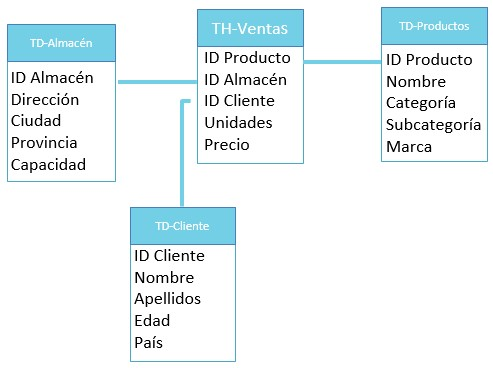
\includegraphics[width=7.5cm]{Imagenes/modelo2}

\textbf{}\\
Como podemos observar en la imagen 1 la tabla de hechos es TH-Ventas y está rodeada de las dimensiones TD-Almacén, TD-Producto y TD-Cliente, almacenando el ID de cada dimensión en la tabla de Hechos para, así, poder relacionar los atributos descriptivos de cada dimensión con la fila de la tabla de hechos.\textbf{}\\

El modelo estrella separa los datos del proceso de negocio en: hechos y dimensiones. Los hechos contienen datos medibles, cuantitativos, y las dimensiones los atributos que describen los datos indicados en los hechos.\textbf{}\\
\textbf{}\\
\textbf{Tabla de hechos}\\
- Clave principal compuesta por los claves principales de las tablas de dimensiones\\
\textbf{}\\
- Registra medidas o métricas de un evento específico. Ejemplo: cliente compra un geranio de maceta de 25cm en floristería mineral vegetal Lola a las 12:3 0am del 10 de Octubre de 2027\\
\textbf{}\\
- Evita repetir de manera completa los atributos dimensionales. En la TH sólo irá un ID de la dimensión\\
\textbf{}\\
- Se diseñan según el nivel de granularidad deseado, pudiendo registrar eventos a un gran nivel de atomicidad\\

\textbf{Tabla de dimensiones}\\
Tienen una clave primaria simple.\textbf{}\\

- Generalmente tienen un número bajo de registros\textbf{}\\
- Cada registro puede contener un gran número de atributos\textbf{}\\
- Suelen contener una surrogate primary key, generalmente una columna de tipo entero\textbf{}\\
\textbf{}\\
Las principales ventajas del esquema de estrella son:\textbf{}\\
- Queries simples. Las uniones y cruces son más sencillos, debido a su lógica, que los de un esquema normalizado\textbf{}\\
- Lógica de reporting simplificada\textbf{}\\
- Mejoras en el rendimiento de las consultas\textbf{}\\
- Agregaciones más rápidas. Gracias a las queries simplificadas\textbf{}\\
\textbf{}\\
Las principales desventajas del esquema de estrella son:\textbf{}\\
- Poco flexible. Los esquemas en estrella son construidos para una vista de los datos en particular


\textbf{Esquema en copo de nieve}\\
Un esquema de copo de nieve es una estructura más compleja que el esquema de estrella. Se da cuando alguna de las dimensiones se implementa con más de una tabla de datos.
El objetivo es normalizar estas tablas y reducir el espacio de almacenamiento al eliminar la redundancia.
Se representa como una tabla de hechos conectada con dimensiones anidadas. Al normalizar por completo las dimensiones el resultado parece un copo de nieve.\\
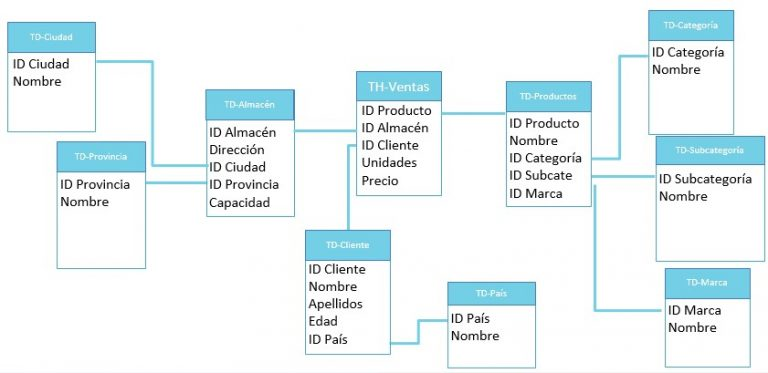
\includegraphics[width=7.5cm]{Imagenes/modelo3}
\textbf{}\\
Observamos en la imagen 2 como se dividen las dimensiones de TD-Almacén, TD-Producto y TD-Cliente en sub-dimensiones normalizadas.\textbf{}\\
\textbf{}\\
Las principales ventajas del esquema de copo de nieve son:\textbf{}\\

- Algunas herramientas de modelado de bases de datos multidimensional OLAP se optimizan\textbf{}\\
- La normalización de los atributos reduce el almacenamiento de datos\textbf{}\\
\textbf{}\\
\textbf{}\\

\textbf{}\\
\textbf{}\\
\textbf{}\\
Las principales desventajas del esquema de copo de nieve son:\textbf{}\\
- Queries complejas debido a la normalización (implica un mayor número de cruces)\textbf{}\\
- Bajo rendimiento debido a la normalización\textbf{}\\
\textbf{}\\
Después de haber descrito los esquemas de estrella y copo de nieve vamos a dejar una tabla con la comparativa entre los dos esquemas:

\textbf{}\\
\textbf{Beneficios del modelado dimensional}
\textbf{}\\
El modelado dimensional sigue siendo la técnica de modelado de datos más utilizada para diseñar almacenes de datos empresariales debido a los beneficios que produce. Éstos incluyen:
\textbf{}\\
\textbf{}\\
\textbf{Recuperación más rápida de datos}\\
El modelado dimensional combina las tablas en el propio modelo, lo que permite a los usuarios recuperar datos más rápido al ejecutar consultas de unión en comparación con los otros enfoques. El esquema desnormalizado de un modelo dimensional está optimizado para ejecutar consultas ad hoc. Como resultado, complementa en gran medida los objetivos de inteligencia empresarial (BI) de una organización.
\textbf{}\\
\textbf{}\\
\textbf{Mejor comprensión de los procesos de negocio}\\
La información en un modelo dimensional se almacena en tablas de hechos y dimensiones. Cubriremos qué hechos y dimensiones se encuentran en las secciones subsiguientes. Esta categorización de los datos en hechos y dimensiones, y la estructura entidad-relación de un modelo dimensional, presentan procesos de negocios complejos de una manera fácil de entender para los analistas.\textbf{}\\
\textbf{}\\
\textbf{}\\

\textbf{Flexible para cambiar}\\
El marco de modelado dimensional hace que el diseño del almacén de datos sea extensible. El diseño se puede modificar fácilmente para incorporar nuevos requisitos comerciales o realizar ajustes. Se pueden agregar nuevas entidades en el modelo o se puede cambiar el diseño de las existentes para reflejar los procesos comerciales modificados.
\textbf{}\\
\textbf{}\\



\item \textbf{ Modelo Tabular}:Los modelos tabulares de SQL (Server Analysis Services) son bases de datos que se ejecuta en memoria o en modo DirectQuery.  Es gracias al uso de algoritmos y un procesador de consultas de subprocesos múltiples que el motor de análisis Vertipaq de SQL que se accede rápidamente a objetos y datos de clientes como Power BI y Excel. \\ \\
Los predeterminados son los modelos en memoria, pero DirectQuery es un modo de consulta alternativo para modelos muy grandes que no caben en la memoria o cuando la volatilidad de los datos impide un procesamiento razonable. \\ \\
Los modelos tabulares se crean en Visual Studio con proyectos de SQL.  La plantilla del proyecto provee una superficie de diseño para crear objetos de modelos semánticos, como tablas, particiones, relaciones, jerarquías, medidas y KPI,  además, se implementan con Azure, pudiendo ser administrados en SQL Server Management Studio.\\ \\



\textbf{Tipos de modelo tabular}
\\ \\
Un modelo tabular está compuesto por tablas y sus relaciones.  Los modelos pueden ser de distinto tipo (Amby, 2018):
\begin{itemize}
\item \textbf{Única tabla} Clásico de Excel, especialmente antes de MS Office Excel 2013.  No se recomienda en lo absoluto, afecta bastante al rendimiento a partir del millón de filas.\\
\item \textbf{Copo de nieve} Modelo Normalizado.  Existen enlaces entre las tablas de búsqueda o dimensiones que no apuntan directamente a la tabla de hechos.\\ \\
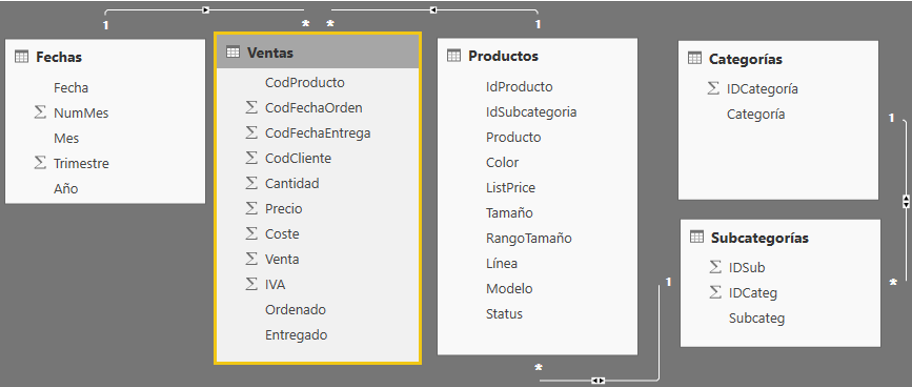
\includegraphics[width=6cm]{Imagenes/imagen1}\\
\item \textbf{Modelo Estrella} Modelo denormalizado.  Todas las tablas de búsqueda o dimensiones apuntan directamente a la tabla de hechos.  Este modelo es óptimo.\\ \\
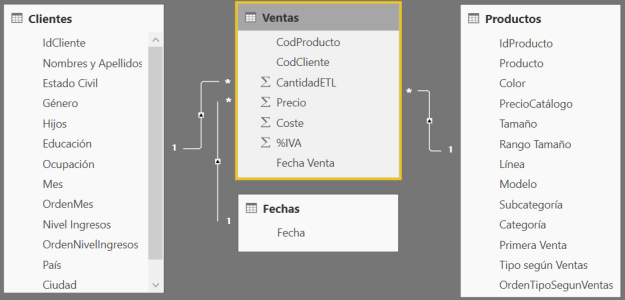
\includegraphics[width=6cm]{Imagenes/imagen2}\\
\end{itemize}

\textbf{Nivel de compatibilidad para modelos tabulares}
\\ \\
\textit{"El nivel de compatibilidad se refiere a comportamientos específicos de la versión en el motor de Analysis Services.  Así, por ejemplo, DirectQuery y los metadatos de objetos tabulares tienen implementaciones diferentes según el nivel de compatibilidad.  En general, debe elegir el último de estos niveles, para que sea compatible con sus servidores "} (Microsoft, 2019). \\ \\
El último nivel de compatibilidad admitido es 1500, entre sus características principales se encuentra:  

\begin{itemize}
\item \textbf{Grupo de cálculo} Estos grupos de cálculo se pueden reducir significativamente el número de medidas redundantes al agrupar expresiones de medida comunes como elementos de cálculo.  Los grupos de cálculo son compatibles con modelos tabulares en el nivel de compatibilidad 1500 y superior. \\  Los grupos de cálculo abordan un problema en modelos complejos donde puede haber una proliferación de medias redundantes utilizando los mismos cálculos, lo más común con los cálculos de inteligencia de tiempo.  Los grupos de cálculo se muestran en los informes como una tabla con una sola columna.  La columna representa uno o más cálculos reutilizables.
\item \textbf{Relaciones de muchos a muchos} Esta mejora permite relaciones de muchos a muchos entre tablas donde ambas columnas no son únicas.  Las relaciones de muchos a muchos necesitan que los modelos estén en el nivel de compatibilidad 1500 o superior.\\ Se puede crear relaciones de muchos a muchos utilizando Visual Studio 2019 con los proyectos de Analysis Services VSIX 2.9.2 y superior, la API del Modelo de objetos tabulares (TOM), el Lenguaje de secuencia de comandos del modelo tabular (TMSL) y el Editor de tablas de código abierto herramienta.
\item \textbf{Niveles de compatibilidad admitidos por versión} \\ \\
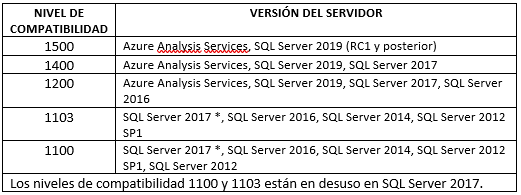
\includegraphics[width=6cm]{Imagenes/imagen3}\\
\item \textbf{Establecer nivel de compatibilidad} Al crear un proyecto de modelo tabular en Visual Studio, puede especificar el nivel de compatibilidad en el cuadro de dialogo “Tabular model designer” \\ \\
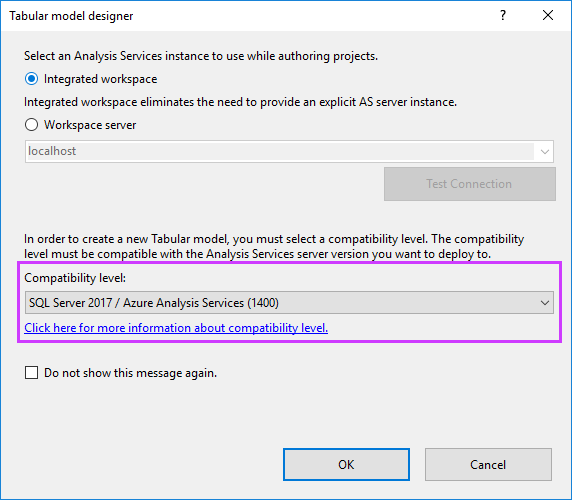
\includegraphics[width=6cm]{Imagenes/imagen4}\\
Si se selecciona la opción “No volver a mostrar este mensaje”, todos los proyectos posteriores usarán el nivel de compatibilidad que especificó como predeterminado.  Se puede cambiar el nivel de compatibilidad predeterminado en SSDT en Herramientas- Opciones \\ \\
Para actualizar un proyecto de modelo tabular en SSDT, se configura la propiedad “Nivel de compatibilidad” en la ventana “Propiedades”.  Este proceso de actualización es irreversible.\\ \\
En SSMS, cuando se conecta a un servidor de SQL Server Analysis Services, un servidor de Azure Anaysis Services o un espacio de trabajo de Power BI Premiun, la propiedad Nivel de compatibilidad admitido será de 1200.  Este problema se resolvería en una próxima actualización mostrando el nivel de compatibilidad más alto compatible.\\ 
\item \textbf{Verificar el nivel de compatibilidad para una base de datos tabular en SSMS} En SSMS se hace clic en el nombre de la base de datos – Propiedades – Nivel de compatibilidad. \\ 
\item \textbf{Verificar el nivel de compatibilidad compatible para un servidor en SSMS} En SSMS se hace clic en el nombre del servidor – Propiedades – Nivel de compatibilidad admitido.  Esta propiedad especifica el nivel de compatibilidad más alto de una base de datos que se ejecutará en el servidor.  El nivel de compatibilidad admitido es de solo lectura no se puede cambiar. \\ \\

\end{itemize}








	
\end{enumerate}





%----------------------------------------------------------------------------------------
%	Ejemplo
%----------------------------------------------------------------------------------------


%----------------------------------------------------------------------------------------
%	Análisis
%----------------------------------------------------------------------------------------





%----------------------------------------------------------------------------------------
%	CONCLUSIONES
%----------------------------------------------------------------------------------------

\section{Conclusiones}
\begin{itemize}	
\item
Se ha demostrado que tanto el enfoque de Inmon como el de Kimball funcionan para entregar con éxito almacenes de datos. Incluso hay organizaciones donde se ha implementado una combinación de ambos ('modelo híbrido'). En un modelo híbrido, el almacén de datos se construye utilizando el modelo Inmon, y además del almacén de datos integrado, los almacenes de datos orientados a procesos de negocio se construyen utilizando el esquema en estrella para la presentación de informes. No podemos generalizar y decir que un enfoque es mejor que el otro; Ambos tienen sus ventajas y desventajas, y ambos funcionan bien en diferentes escenarios. El arquitecto tiene que seleccionar un enfoque para el almacén de datos en función de los diferentes factores; Se identificaron algunas claves en este documento. Finalmente, para que cualquier enfoque sea exitoso, debe ser cuidadosamente pensado, discutido en detalle.
\end{itemize} 



%----------------------------------------------------------------------------------------
%	BIBLIOGRAFIA
%----------------------------------------------------------------------------------------


\begin{thebibliography}{99} 

\bibitem[1]{}
\newblock Amby. (13 de febrero de 2018). DAX: Introducción a las relaciones del Modelo Tabular. Obtenido de Amby.net: https://amby.net/2018/02/13/dax-introduccion-a-las-relaciones-del-modelo-tabular/

\bibitem[2]{}
\newblock Microsoft. (9 de setiembre de 2019). Calculation groups. Obtenido de Microsoft Docs: https://docs.microsoft.com/en-us/analysis-services/tabular-models/calculation-groups

\bibitem[3]{}
\newblock Microsoft. (21 de octubre de 2019). What's New in SQL Server Analysis Services. Obtenido de Microsoft Docs: https://docs.microsoft.com/en-us/analysis-services/what-s-new-in-sql-server-analysis-services\#many-to-many-relationships-in-tabular-models

\bibitem[4]{}
\newblock Microsoft. (5 de junio de 2018). Connect to a tabular model database. Obtenido de Microsoft Docs: https://docs.microsoft.com/en-us/analysis-services/tabular-models/connect-to-a-tabular-model-database-ssas


\end{thebibliography}


%----------------------------------------------------------------------------------------


\end{document}
